% FEUP THESIS STYLE for LaTeX2e
% how to use feupteses (changed from the original for MIEEC)
%
% FEUP, JCL & JCF, Tue May 20 18:53:15 2008
%
% PLEASE send improvements to jlopes at fe.up.pt, jcf at fe.up.pt
%

%%========================================
%% Commands: pdflatex mieic
%%           bibtex mieic
%%           makeindex mieic (only if crating an index) 
%%           pdflatex mieic
%%========================================

%% For one side layout comment next line and uncomment the second line
\documentclass[11pt,a4paper,twoside,openright]{report}
%\documentclass[11pt,a4paper]{report}

%% For iso-8859-1 (latin1), comment next line and uncomment the second line
\usepackage[utf8]{inputenc}
%\usepackage[latin1]{inputenc}

%% Use option portuges if needed
\usepackage[english]{babel}

%% For the final version, comment next line and uncomment the second line
%\usepackage[provisional,alpharefs]{feupteses}      
\usepackage[alpharefs]{feupteses} 

%% Options: 
%% - portuges: titles, etc in portuguese
%% - provisional: the thesis has not been approved yet
%% - usewatermark: use watermark instaed of provisonal text
%% - print: links are not shown (for paper versions)
%% - alpharefs: bibliography references are alphabetic
%% - numericrefs: bibliography references are numbered (in order of citation)
%% ( by default: author-date format of the ``natbib'' package is used 
%%   the portuguese version requires the file ``plainnat-pt.bst'' to be 
%%   present in the same directory )

%% Include MIEIC definitions different from standard style
\usepackage{mieicpatch}

%% Package to allow footnotes in floats
\usepackage{fmtcount}

% % insert source code
\usepackage{listings}
\usepackage{color}

\usepackage[nodayofweek,12hr]{datetime}

%% Provide a version number in order to keep track of
%% thesis versions (it will printed in the footer of most pages)

\version{1.0}

%% Uncomment in the final version in order to make version footer disappear
\noversiontrue                 

%% Uncomment to create an index (at the end of the document)
%\makeindex                      

%% Path to the figures directory
%% TIP: use folder ``figures'' to keep all your figures
\graphicspath{{figures/}}       

%%----------------------------------------
%% TIP: if you want to define more macros, use an external file to
%% keep them
%some macro definitions

% format
\newcommand{\class}[1]{{\normalfont\slshape #1\/}}

% entities
\newcommand{\Feup}{Faculdade de Engenharia da Universidade do Porto}

\newcommand{\svg}{\class{SVG}}
\newcommand{\scada}{\class{SCADA}}
\newcommand{\scadadms}{\class{SCADA/DMS}}


% \myfigure{file}{caption}
\newcommand{\myfigure}[2]{\mycustomfigure{#1}{#2}{width=0.86\textwidth}}

% \mycustomfigure{file}{caption}{params}
\newcommand{\mycustomfigure}[3]{\mycustomcaptionfigure{#1}{#2}{#3}{#2}}

\newcommand{\mycustomcaptionfigure}[4]{\begin{figure}[t]
  \begin{center}
    \leavevmode
    \includegraphics[#3]{#1}
    \caption[#4]{#2}
    \label{fig:#1}
  \end{center}
\end{figure}}

% \mycustomfigure{file}{caption}{params}
\newcommand{\myoriginalfigure}[2]{\begin{figure}[t]
  \begin{center}
    \leavevmode
    \includegraphics{#1}
    \caption{#2}
    \label{fig:#1}
  \end{center}
\end{figure}}

% \myfigure{label}{caption}{table spec}{contents}
\newcommand{\mytable}[4]{\begin{table}[t]
  \footnotesize
  \centering
  \caption{#2}
  \begin{tabular}{#3}
    #4
  \end{tabular}
  \label{tab:#1}
\end{table}}

\newcommand{\myprinciple}[7]{
  \mytable{#1}{#2}{p{2cm}|p{12cm}}{
  \hline Name & #3 \\ 
  \hline Statement & #4 \\ 
  \hline Rationale & #5 \\
  \hline Implications & #6  \\ 
  \hline 
}} 

\newcommand{\mysummary}[5]{
\mytable{#1}{#2}{p{1.8cm}||p{6cm}|p{6cm}}{
\hline & \textbf{Recent developments} & \textbf{Future vision} \\ \hline
\hline \textbf{Application Architecture} & #3 \\ 
\hline \textbf{Information Architecture} & #4 \\ 
\hline \textbf{Technical Architecture} & #5
}}

%%----------------------------------------

%%========================================
%% Start of document
%%========================================
\begin{document}

%%----------------------------------------
%% Information about the work
%%----------------------------------------
\title{Information Systems Architecture definition for the Electronic Health Record (EHR)}
\author{Eduardo Filipe Garcia Pinto}
\degree{Master in Informatics and Computing Engineering}
%% Date of submission
\thesisdate{\today}

%% Insert copyright text if used
%\copyrightnotice{Name of the Author, 2008}

\supervisor{Supervisor}{António Carvalho Brito}{(PhD)}
%% Uncomment next line if necessary
%\supervisor{Second Supervisor}{Name of the Supervisor}{(Title)}

%% Uncomment committee stuff in the final version
%\committeetext{Approved in oral examination by the committee:}
%\committeemember{Chair}{Name of the President}{(Title)}
%\committeemember{External Examiner}{Name of the Examiner}{(Title)}
%\committeemember{Supervisor}{Name of the Supervisor}{(Title)}
%\signature
%\committeedate{31$^{st}$ July, 2010}

%% Specify cover logo (in folder ``figures'')
\logo{feup-logo.pdf}

%%----------------------------------------
%% Cover page(s)
%%----------------------------------------
\maketitle

%% Uncomment next line in the final version
\committeepage
%MIEEC uses an external PDF page with the signatures (juri.pdf)
%\includepdf[pagecommand={},noautoscale=false,fitpaper=true,pages=-]{juri.pdf}

%% Preliminary materials
\StartPrelim
\begin{singlespace}
  \chapter*{Abstract}

The Information Technologies have revolutionized many areas of society. Since many years ago, the health area has been searching for solutions to improve existing processes, having as the main objective the improvement of healthcare services. In this sense, the availability of patient clinical data can be vital to a more effective diagnosis and treatment, by a health professional. This information should be accessible regardless of context, place, time or where it was collected. In order to share this type of data, many countries have initiated projects implementing Electronic Health Record (EHR), including Portugal in 2010.

The EHR complexity and scope makes it an high cost and risk project. In fact, the inherent difficulties of a project like this are as critical as its importance and the impact it has on societies. The implementation of a successful EHR implies, in most cases, the involvement of all stakeholders, from patient to health organizations, along with the professionals themselves, becoming a very long and continuous process.

In the context of this dissertation we pretend to build a architecture proposal for implementing the Portuguese EHR. The proposed architecture should serve as a platform for sharing information between multiple health entities, normalizing processes, applying conventions and chasing interoperability among agents. The ability of the system evolution on one hand, and ease of integration in international projects on the other, are two major concerns to be taken into account throughout the proposal definition process.

This document reflects the study in order to understand what processes and practices are used in implementing these large-scale projects. Accordingly, we present some models of enterprise architectures as well as some architectural styles, both corresponding to high levels of abstraction. Regarding the integration of different systems, this document addresses several international conventions for transmission, encoding and storing of clinical information, such as HL7, openEHR and SNOMED CT. Also, we briefly analyse two International EHR case studies, in UK and Canada. In conclusion it should be noted that regardless of the technical challenges that may arise, the process must always be guided by the objective of improving healthcare services to the patient.

\section*{}
\textbf{Keywords:} Electronic Health Record; Health Information Systems; Interoperability; Information Systems Architecture

\chapter*{Resumo}

As Tecnologias de Informação têm revolucionado as mais diversas áreas da sociedade. Desde há muitos anos atrás, a área da saúde tem procurado soluções tecnológicas que permitam melhorar os processos existentes, tendo como principal objetivo a melhoria dos cuidados de saúde que são prestados. Neste sentido, a disponibilidade da informação clínica sobre um paciente pode ser vital para um diagnóstico e tratamento mais eficazes, por parte de um profissional de saúde. Esta informação deve estar acessível independentemente do contexto, local ou data onde foi coletada. Com o objetivo de providenciar este tipo de dados, muitos países iniciaram projectos de implementação de Registo de Saúde Electrónico (RSE), entre os quais se inclui Portugal, em 2010. 

A complexidade e abrangência faz do RSE um projecto de altos custo e risco. De facto, as dificuldades inerentes a um projecto deste género fazem juz à sua importância e ao impacto que tem nas sociedades. A implementação com sucesso de um RSE é um processo longo e implica, na maioria dos casos, o envolvimento de todos os agentes intervenientes no processo, desde o paciente à instituição de saúde, passando pelos próprios profissionais.

No contexto desta dissertação pretende-se construir uma proposta de arquitectura para implementação do RSE em Portugal. A arquitectura proposta deve servir como uma plataforma de partilha de informação entre as mais diversas entidades de saúde, nor\-ma\-li\-zan\-do os processos e codificações nesta área e promovendo a interoperabilidade entre os agentes. A capacidade de evolução do sistema por um lado, e a facilidade de integração em projectos internacionais por outro, são duas grandes preocupações a ter em conta ao longo do processo de definição da proposta.

O presente documento reflecte o estudo feito no sentido de perceber quais os processos e práticas existentes na implementação destes projectos de larga escala. Nesse sentido, apresentam-se alguns modelos de arquitecturas empresariais assim como alguns estilos de arquitectura, ambos correspondentes a níveis de elevada abstracção. No que diz respeito à integração de diferentes sistemas, são abordadas diversas convenções internacionais para transmissão, codificação e armazenamento da informação clínica, como o HL7, SNOMED CT ou openEHR. Ainda no âmbito deste documento, são analisados dois casos de estudo internacionais do RSE, no Reino Unido e no Canadá. Para concluir, importa sublinhar que, independentemente dos desafios técnicos que se possam apresentar, o processo deve ser sempre guiado pelo objectivo principal de melhorar os cuidados de saúde ao paciente.

\section*{}
\textbf{Palavras-chave:} Registo de Saúde Eletrónico; Sistema de Informação da Saúde; Interoperabilidade; Arquitectura de Sistemas de Informação

%O Resumo fornece ao leitor um sumário do conteúdo da dissertação.
%Deverá ser breve mas conter detalhe suficiente e, uma vez que é a porta
%de entrada para a dissertação, deverá dar ao leitor uma boa impressão
%inicial.
%
%Este texto inicial da dissertação é escrito no fim e resume numa
%página, sem referências externas, o tema e o contexto do trabalho, a
%motivação e os objectivos, as metodologias e técnicas empregues, os
%principais resultados alcançados e as conclusões.
 % the abstract
  %\chapter*{Acknowledgements}

To all of those who contributed in some how to the success of this dissertation work.

\vspace{10mm}
\flushleft{Eduardo Pinto}
  % the acknowledgments
  \cleardoublepage
\thispagestyle{plain}

\vspace*{8cm}

\begin{flushright}
   \textsl{``You should be glad that bridge fell down. \\
           I was planning to build thirteen more to that same design''} \\
\vspace*{1.5cm}
           Isambard Kingdom Brunel
\end{flushright}
    % initial quotation if desired
  \cleardoublepage
  \pdfbookmark[0]{Table of Contents}{contents}
  \tableofcontents
  \cleardoublepage
  \pdfbookmark[0]{List of Figures}{figures}
  \listoffigures
%  \cleardoublepage
%  \pdfbookmark[0]{List of Tables}{tables}
%  \listoftables
  \cleardoublepage
  \pdfbookmark[0]{Abbreviations}{abbrevs}
  \chapter*{Abbreviations}
\chaptermark{ABBREVIATIONS}

\begin{flushleft}
\begin{tabular}{l p{0.8\linewidth}}
ACES	& Agrupamentos de Centros de Saúde (Healthcare Primary Institutions Groups) \\
ADL		& Archetype Definition Language \\
ADM		& Architecture Development Method \\
ANSI	& American National Standards Institute \\
ARS		& Administração Regional de Saúde (Health Regional Administration) \\
ARSN	& Administração Regional de Saúde do Norte (Health Regional Administration of North) \\
CBSS	& Community-Based Service Systems \\
CDA		& Clinical Document Architecture \\
CIC		& Comissão para a Informatização Clínica (Commission for Clinical Informatics) \\
CNPD	& Comissão Nacional de Proteção de Dados (National Committee for Data Protection) \\
CSP		& Cuidados de Saúde Primários (Primary Healthcare Services) \\
DICOM	& Digital Imaging and Communications in Medicine \\
ECS		& Emergency Care Summary \\
EDA		& Event-driven Architecture \\
EHR		& Electronic Health Record \\
EMR		& Electronic Medical Record \\
FEAF	& Federal Enterprise Architecture Framework \\
FEUP	& Faculty of Engineering of University of Porto \\
GP		& General Practitioner \\
HIS		& Health Information Systems \\
HL7		& Health Level 7 \\
ICD		& International Classification of Diseases and Related Health Problems \\
IHE		& Integrating Healthcare Enterprise \\
IHTSDO  & International Health Terminology Standards Development Organisation \\
IS		& Information Systems \\
ISO		& International Standardisation Organization \\
IT		& Information Technology \\
LOINC   & Logical Observations Identifiers Names and Codes \\
NHS		& National Health Service \\
OSS		& Open-source Systems \\
PDS		& Plataforma de Dados da Saúde (Healthcare Data Platform) \\
PS		& Patient Summary \\
RIM		& Reference Information Model \\
RIS		& Rede de Informação da Saúde (Health Information Network) \\
RNU		& Registo Nacional de Utentes (Patients National Record) \\
SCR		& Summary Care Record
\end{tabular}
\end{flushleft}

\begin{flushleft}
\begin{tabular}{l p{0.8\linewidth}}
SINUS	& Sistema de Informação de Unidades de Saúde (Information System for Health Institutions)\\
SNOMED	& Systematized Nomenclature of Medicine \\
SOA		& Service-oriented Architecture \\
SOAP	& Simple Object Access Protocol \\
SONHO	& Sistema Integrado de Informação Hospitalar (Integrated System for Hospital Information) \\
TOGAF   & The Open Group Architecture Framework \\
WHO		& World Health Organization \\
XACML	& eXtensible Access Control Markup Language \\
XML	    & Extensible Markup Language \\
ZF		& Zachman Framework 
\end{tabular}
\end{flushleft}  % the list of abbreviations used
\end{singlespace}

%%----------------------------------------
%% Body
%%----------------------------------------
\StartBody

%% TIP: use a separate file for each chapter
\chapter{Introduction} \label{chap:intro}

\section*{}

%O primeiro capítulo da dissertação deve servir para apresentar o
%enquadramento e a moti\-va\-ção do trabalho e para identificar e
%definir os problemas que a dissertação aborda.
%Deve resumir as metodologias utilizadas no trabalho e termina
%apresentando um breve resumo de cada um dos capítulos
%posteriores.

%\begin{quote}
%  ``Like the Abstract, the Introduction should be written to engage the
%  interest of the reader. It should also give the reader an idea of
%  how the dissertation is structured, and in doing so, define the
%  thread of the contents.''~\citepp[chap.\ Introduction]{kn:Tha01} 
%\end{quote}


The revolution and advent of technology has been changing the way people interact with each other, forcing the companies to adopt new business strategies, improving life's quality and so forth. In the organizations' context, the Information Systems brought a new opportunity for improving and optimizing processes, helping to generate value and profits and making them more competitive~\citep{Gurbaxani1991}.

The health context is one of the most complex and critical, compelling the organizations to support several business processes and interacting with multiple stakeholders from clinicians to laboratory technicians. With such a complex scenario it seems easy to understand the impact that the technology might have, automating processes or sharing information among all the interested parties. However, this complexity obviously raises the risks of failing for projects implementation, either because the products do not meet the requirements, the stakeholders' expectations or were built excessively monolithic what preclude future integration and evolution~\citep{Chu2006}.

\section{Background} \label{sec:background}

Despite of the healthcare arena largeness and the inherent difficulties of comprehensive Information Technology (IT) projects, several concepts and platforms started appearing~\citep{Haux2006}. For instance, seems reasonable to say that the patient clinical information should be available to its consumers when needed, whatever the place or time of the occurrence. The Electronic Health Record (EHR) concept is described~\citep{Gunter2005} as the ``longitudinal collection of electronic health information about individual patients and populations''. The main objective is to provide clinical information about a patient where it needs to be consulted, independently of its origin or location, helping to avoid clinical errors or duplication of efforts and resources. It is supposed to be a mechanism for integrating healthcare information for the purpose of improving care quality~\citep{Orszag2008} but obviously, these EHR systems are as complex as the implementations challenges they face.

%Esta secção descreve a área em que o trabalho se insere, podendo
%referir um eventual projecto de que faz parte e apresentar uma breve
%descrição da empresa onde o trabalho decorreu.
\section{Context} \label{sec:context}

The benefits of an EHR seem consensual and undeniable. All around the world, several countries started expensive programmes trying to implement partial or total EHR solutions, some being more successful than others.

The Portuguese health information systems suffer from the same problems~\citep{Deloitte2011} that probably most of the countries: all over the years, the systems were being created essentially to solve local problems. These systems were developed without any kind of concern about interoperability --- designing and building the systems following standards and not precluding future communications and data sharing. The consequence is quite predictable: the multiple existing systems, which have many purposes, use different codification standards and several interfaces to allow communication, do not have the capability to ``talk'' with each other. Plus, even if they could communicate, they would not be able to understand each other since they do not use the same language to express themselves. As final consequence, there is a huge amount of clinical data that cannot be shared.

In 2010, the Ministry of Health signed a protocol with the Faculty of Engineering of University of Porto (FEUP) establishing a partnership for delivering some recommendations about the design and implementation for the EHR. This dissertation appears under the scope of that protocol.

%Apresenta a motivação e enumera os objectivos do trabalho terminando
%com um resumo das metodologias para a prossecução dos objectivos.
\section{Motivation and Objectives} \label{sec:goals}

Clements, Kazman and Klein advocate~\citep{Clements2001} that ``architectures allow or preclude nearly all the system's quality attributes''. In this sense, when it is pretended to create a system where the quality attributes are critical, the architecture is certainly one of the most relevant means to assure and facilitate them.

The purpose of this dissertation is to build an architecture proposal to the Portuguese EHR. This architecture must allow the integration of the existing multiple Health Information Systems, as well as providing an infrastructure for sharing data. The proposal must promote the interoperability between different healthcare organizations, either by forcing the utilization of international standards and conventions or by establishing well-defined interfaces. The future evolution of the system must also be taken into account when designing the architecture proposal.

Despite the deliverable is an architecture proposal, the final objectives can be pointed out as follows:
\begin{itemize}
\item deliver an architecture proposal, able to offer a complete and integrated vision from the healthcare organization level to the EHR level;
\item development a set of recommendations that fosters interoperability and sharing of clinical information between different healthcare institutions;
\item describe the necessary changes in the applications architecture in order to allow new services integration and facilitate the creation of an EHR system.
\end{itemize}

The thesis research was done through a straight collaboration with the Ministry of Health, allowing to work close to the EHR stakeholders. In this sense, the weekly meetings with the responsible entities were used to discuss the main architectural issues.


\section{Document Structure} \label{sec:struct}

In the present chapter we described the context, motivation and goals of this dissertation. The document has more 5 chapters:
\begin{itemize}

\item Chapter~\ref{chap:inf-sys}, \textit{Information Systems Models and Frameworks} -- small introduction about the HIS and try to understand what kind of methodologies may be used to facilitate the implementation of such large systems, using Enterprise Architectures. Then, we briefly describe three Architectural Styles which stand as excellent solutions to solve some kind of architecture issues;

\item Chapter~\ref{chap:standards}, \textit{International Practices and Conventions} -- description of some of the health international standards trying to understand what advantages one has and where should each one be adopted. Next, we overview the implementation of two EHR case studies, in England and in Canada;

\item Chapter~\ref{sec:struct_concepts}, \textit{Structural Concepts and Architecture} -- clarification of some essential concepts to the research as well as to characterise the actual situation and organisation of the national healthcare public service;

\item Chapter~\ref{chap:arch-proposal}, \textit{Architectural Contributions} -- description of the contributions done in the scope of the thesis. It starts with the presentation of five principles followed by the detailed contribution to each project defined by the responsible entities;

\item Chapter~\ref{chap:concl}, \textit{Conclusions} -- state some final considerations about the work done. It reflects about the problems that appeared and the solutions adopted and perspectives the mid-term future for the Portuguese healthcare system.

\end{itemize}


Despite the document is written in English, there will be some concepts that shall not be translate since they represent entities or project names. In that case, the first time it appears its literal translation will be inserted as a footnote. 
\chapter{Information Systems Models and Frameworks} \label{chap:inf-sys}

\section*{}

%Neste capítulo é descrito o estado da arte e são
%apresentados trabalhos relacionados para mostrar o que existe no
%mesmo domínio e quais os problemas em aberto.
%Deve deixar claro que existe uma oportunidade de desenvolvimento que
%cobre alguma falha concreta .
%
%O capítulo deve também efectuar uma revisão tecnológica às principais
%ferramentas utilizáveis no âmbito do projecto, justificando futuras
%escolhas.


%\section{Health Information Systems}
%
%\subsection{Information Systems}
%
%%Falar sobre os sistemas de informação de forma genérica
%
%\subsection{Portugal overview}\label{sec:dialecto}
%

In this chapter we present a general study about how is it possible to build ultra-large systems. The Information Systems (IS) are a kind of large dimension systems. The development methods used to implement these systems are an important source of experiences and techniques relevant to this dissertation. The first section describes some Enterprise Architecture Frameworks and in the second one we introduce two Architectural Models.


\section{Enterprise Architecture Frameworks} \label{sec:ea-frams}
The concept of Enterprise Architecture appeared more than 20 years ago. At that time, the systems complexity was growing with an exponential velocity. However, most of the times, those systems were not able to fulfil the business needs and the problem was not lack of technology or knowledge but difficulties in understanding the business from those who were developing it. Thus, the software development was facing two problems at a time: in one hand, the systems were becoming huge and hugely complex; on the other hand, the systems were developed with few concerns about business orientation~\citep{Sessions2007}.

Despite of being a problem with a considerable age and very studied also, it did not stop growing and there is not a quite clear solution. A lot of enterprise architecture models appeared and disappeared over the years. However, it is estimated that around 90\% of the market is dominated by this four methodologies~\citep{Sessions2007}:

\begin{itemize}
\item The Zachman Framework;
\item The Open Group Architecture Framework (TOGAF);
\item The Federal Enterprise Architecture Framework (FEAF);
%TODO \item The Gartner Methodology.
\end{itemize}

In the next subsections, we will slightly describe each one of them, trying to understand which the advantages and weak points of each one. 











\subsection{The Zachman Framework} \label{sec:zachman-fw}

The Zachman Framework~\citep{Zachman1987} aims to guarantee that all stakeholders perspectives are being taken into account when developing a complex software system. In general terms, it is important to understand if all the artefacts are sufficiently focused and if the existing artefacts clarify all the players, from the business owner till the database designer, keeping all the visions aligned.

In the original article and in order to explain his methodology, John Zachman uses an analogy between building an information system and construct a building. Thus, when constructing a building, the architect starts with understanding the general requirements as how many divisions it is supposed to have and the general purpose of the building, usually by using bubble charts. In a second phase, the architect's drawings aims to represent the links between each room of the building and also its general structure. Finally, the architect presents the plans and they must represent and reflect the customer requirements and expectations. These plans already include several details about electrical system, masonry, wood structure, etc. After plans arrive the contractor, they suffer some adjustments either because of costs/price or because another kind of constructing limitations.

In general, we can say that there are three fundamental architectural representations, one for each player in this process: the owner, the designer and the builder. Through all this process, the project will be documented in many perspectives. The architect starts listening to the customer and building his own perspective of the project that is sent to the builder, which in turn builds another view that allows himself to clarify some aspects. Despite of all these documents refer and describe the same project, each one of them has different purposes. Each one of them is unique and independent, describes one area, one perspective, not being possible from one of those to conclude about the others.

Originally, the proposal of Zachman was based on a policy of three questions: What?, How? and Where?, used to describe the product. However, the model has evolved and now it is based in three more questions: Who?, When? and Why?.

\addtocounter{footnote}{1}
\begin{figure}[t]
\centering
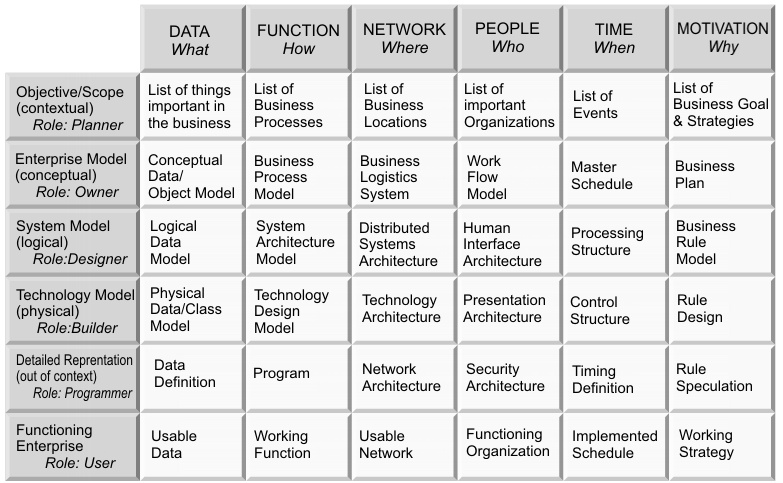
\includegraphics[width=1.0\textwidth]{zachman-framework}
\caption[Zachman Framework classification model]%
			{Zachman Framework classification model$^{\decimal{footnote}}$}
\label{fig:zachman-architecture}
\end{figure}

Just as it is possible to see in Figure~\ref{fig:zachman-architecture}, Zachman claims a classification of the existing artefacts from multiple points of view, identifying:
\begin{itemize}
\item \textbf{Material description} --- the data model of the system: ``entity - relationship - entity''; 
\item \textbf{Functional description} --- the process model of the system: ``input - process - output'';
\item \textbf{Location description} --- the network model of the system: ``node - line - node'';
\item \textbf{People description} --- the organization units and roles within the system: ``organization - reporting - organization'';
\item \textbf{Time description} --- the events of the system: ``event - cycle - event'';
\item \textbf{Motivation description} --- the high level organization goals of the system: ``node - line - node''.
\end{itemize}

\footnotetext[\value{footnote}]{Source: \url{http://upload.wikimedia.org/wikipedia/commons/d/da/Zachman_Framework_Detailed.jpg}}

%A forma como os três intervenientes vê cada entidade do sistema retrata-se também no artigo. De facto, quando o cliente se refere a um empregado está a referir-se à pessoa enquanto que o constructor está a pensar num registo no sistema, dessa entidade.

Over the years, this model started to be considered more like a taxonomy model, helping to frame all the artefacts and state their value and meaning to the multiple stakeholders~\citep{Sessions2007}.






\subsection{The Open Group Architecture Framework} \label{sec:togaf}

First developed in 1995, The Open Group Architecture Framework was based on the US Department of Defense Technical Architecture Framework for Information Management (TAFIM). From this sound foundation, The Open Group Architecture Forum has developed successive versions of TOGAF at regular intervals and published them on The Open Group public web site~\citep{Josey2011}.

TOGAF might be seen as a process for building an Enterprise Architecture. This framework states this building process as a continuous process of building multiple architectures from highly generic to highly specific ones, until reaching the organizational architecture level~\citep{Sessions2007}.

This framework splits the EA in four categories: 
\begin{itemize}
\item \textbf{Business Architecture} --- describes processes used by business to meet own goals;
\item \textbf{Application Architecture} --- describes how to build applications from the framework and how to interact with the other ones;
\item \textbf{Data Architecture} --- describes how the information is stored, organized and accessed;
\item \textbf{Technical Architecture} --- describes the hardware and software supporting the applications and their interactions.
\end{itemize}

One of the most important concepts of this framework is the Architecture Development Method (ADM), which stands as a reliable and proven approach for building enterprise architecture descriptions, keeping the progress close to the business specific needs. Actually, it provides an overall process template for architecture development activity and a narrative of each architecture phase, describing each one in terms of objectives, approach, inputs, steps and outputs to the architects~\citep{Leist2006}.

The TOGAF ADM also provides several guidelines and techniques:
\begin{itemize}
\item \textbf{Architecture Content Framework} --- detailed model for architectural work products, including deliverables and artefacts;
\item \textbf{Enterprise Continuum} --- a model for structuring a virtual repository and classify architecture and solution artefacts, tracking how the artefacts evolve and how they can be re-used;
\item \textbf{TOGAF Reference Models} --- two reference models: Technical Reference Model (TRM) and Integrated Information Infrastructure Model (III-RM);
\item \textbf{Architecture Capability Framework} --- a set of templates, guidelines, resources that aim to help the architect establishing some practices within an organization.
\end{itemize}

In overall terms, TOGAF ADM recommends an iterative process for architecture development, not being prescriptive on breadth of coverage, level of details or time horizons. The architect determines those details to fit one specific project. One of the most important characteristics of TOGAF ADM is that, despite of having well-defined phases, it enough flexible to be adapted to the organization and to let architects build the best approach to implement TOGAF~\citep{Tang2004}.









\subsection{Federal Enterprise Architecture Framework} \label{sec:feaf}

The Federal Enterprise Architecture Framework appeared with the objective of serving as a platform for sharing processes, information and documentation among the U.S. Federal Agencies and other government agencies. This framework gathers two main characteristics of the two previous: in on hand, it defines a taxonomy -- similar to the Zachman Framework (Section \ref{sec:zachman-fw}) -- for artefacts classification; on the other hand, it suggests a process for building and implementing the architecture like TOGAF (Section \ref{sec:togaf}) does. 

The FEAF partitions a given `platform' into business, data, applications and technologies architectures, aiming to take those into account when applying the process of implementing the new architecture. Furthermore, the framework is organized in four levels~\citep{Tang2004}:
\begin{itemize}
\item Level I --- the highest level which deals with the architecture drivers or external stimulus fetching the strategic direction of the architecture. It facilitates the transformation from the original architecture to the new one by applying architecture standards and managing the process;
\item Level II --- an analyses of the business goals, direction, principles, strategies and priorities;
\item Level III --- expression of architecture in more detailed view by using business data, applications and technology views to model it;
\item Level IV --- representation of Data Architecture, Application Architecture and Technology Architecture using a combination of Zachman Framework and Spewak's Enterprise Architecture Planning methods.
\end{itemize}

% Success measurement
FEAF also suggests a measurement process, being able to evaluate the maturity the inner organizations are adopting and implementing the enterprise architecture. This evaluation classifies the agencies measuring three essential attributes: 
\begin{itemize}
\item Architectural completion --- the maturity of the architecture itself;
\item Architectural use --- how is the architecture being used to improve efficiency of decision-making;
\item Architectural results --- the benefits brought by the use of the architecture.
\end{itemize}

Based on the analysis of this three attributes, the agencies are then rated in one of three categories: green, yellow and red. 

%Antes de abordar as diferentes recomendações da FEA importa referir alguns conceitos fundamentais: 
%- segmentos: segmentos de missão central (ex: educação para o Min. Educação) e segmentos de serviços de negócio (ex: gestão financeira)
%- serviços empresariais (ex: gestão de segurança)

%Modelos de referência do FEA 
%- modelo de referência de negócio
%- modelo de referência de componentes
%- modelo técnico de referência
%- modelo de referência de dados- modelo de referência de performance

%Processo do FEA
%1) análise arquitectural
%2) definição da arquitectura
%3) estratégia de financiamento e investimento
%4) gestão do planeamento e execução do projecto




%\subsection{Gartner Enterprise Architecture}
%
%Gartner não pode ser descrito nem como um processo taxonómico, nem como um processo, muito menos como uma metodologia completa. Em vez disso, pode definir-se como uma prática. É uma práctica para arquitecturas empresariais realizada por uma empresa de consultadoria, a Gartner.
%  
%Esta prática não se baseia no que a empresa é, mas naquilo que quer ser, nos objectivos que pretende atingir. Acredita-se que o fundamental está em formar uma equipa constituida por pessoas do negócio, especialistas em informação e os responsáveis de implementação. O essencial para por criar neste grupo de pessoas uma visão comum para a empresa.





\section{Architectural Styles} \label{sec:arch-styles}

An Architectural Style is a particular pattern that organizes components and connectors in a particularly form, providing a well-known reliable solution when facing a specific kind of problem~\citep{Kazman}. Each architectural style principle influences some quality attributes in a positive and some other in a negative way. Zheng Qin \textit{et al} define it as ``a solution to solve a certain class of problems which have common quality attributes requirements'', stating also that ``there is no architecture style that is proper for all systems, because every system have different quality attributes requirements''~\citep{Qin2008}. Kim and Garlan advocate~\citep{Kim2010} that these concepts bring a number of significant benefits as they promote design reuse.

\subsection{The Metropolis Model}

Over the last years, two important trends are changing business and society: in one hand, the growing use of shared knowledge to create high-value services and projects; on the other hand, the growing preponderance of services. The business are evolving from a product-oriented perspective to a relation-oriented one. This change of paradigm brought the client to the middle of the business, helping to create value. The greatest examples of this new philosophy are the systems based in communities as Wikipedia or Facebook, that are able to generate profit and value directly from its users.

The Metropolis Model~\citep{Kazman2009} appears as an attempt of describing really huge complex systems built from two basilar concepts: Open-source Software (OSS) and Community-Based Service Systems (CBSS). Despite the growing importance of OSS and CBSS, there will always be some systems that cannot be developed by crowds, either because of the business criticality or for demanding unquestionable security guarantees. The Metropolis Model does not really apply to those systems.

We will start with an explanation of the `crowdsourced systems' and then briefly describe the principles of the Metropolis Model, always following the original article wrote by Rick Kazman and Hong-Mei Chen~\citep{Kazman2009}.

\subsubsection{Crowdsourced Systems}

The Metropolis Model identify its target as the `crowdsourced systems'. This concept includes the kind of systems with some special characteristics:
\begin{itemize}
\item open teams --- meaning that the assumption of having a closed and dedicated team of programmers should be abandoned;
\item `mashability' --- as the capacity of composing and integrating different systems and functionalities since that
the consumption of software by one person or project does not make it less available for consumption by another;
\item conflicting, not knowable requirements --- the requirements emerge from the contributors and the users, making them highly unpredictable and often being in conflict between each other;
\item continuous evolution --- as a consequence of constant changing requirements and distributed resources, these type of systems are never finished nor stable, introducing the `perpetual beta' concept. The development of the project is done through multiple iterations empowering the users with the responsibility of testing and assuring its quality;
\item focus on operations --- the availability of its operations are, most of the times, as critical as their utility and, in that sense, it is not accepted any kind of system downtime (Amazon, eBay or Google are good examples);
\item sufficient correctness --- the notion of `perpetual beta' expresses the idea of acceptance some incompleteness in software (e.g. Wikipedia);
\item unstable resources --- one of the most interesting facts is that, despite of the volatility of people, information and other resources that individually would be useless, when massive congregated are able to create reliable, stable and impressive computational powered systems;
\item emergent behaviours --- frequently, there are behaviours and tendencies that emerge from the system that are completely unexpected. In these systems, unlike the traditional ones, the crowds take the rudder and bring to the system unpredicted kinds of utilization or interaction.
\end{itemize}

\subsubsection{The principles}

The Metropolis Model presents a new unified vision between the CBSS and the OSS, focusing deliberately in the crowd value generation. This model suggests the creation of two levels: the kernel services and the periphery services. It states that the application's kernel may be developed using traditional methods.

The Metropolis Model is supported by the application of some principles:
\begin{itemize}
\item \textbf{Crowd engagement and egalitarian management of open teams} --- the management must focus the people and the crowds, engaging the users for value co-creation. The engagement is not just a system-level issue, but a question of business strategy. These kind of system resort to crowd-sourcing chasing ``potential for cost reduction, increased innovation, and quicker development time for delivering products and services that meet customer needs'' as the authors explain;
\item \textbf{Bifurcated requirements} --- the requirements must be distinguished into kernel or periphery ones. The kernel should ``deliver little or no end-user value'' (e.g. Linux kernel, Wikipedia wiki or Facebook application platform). On the other hand, from the periphery appears most of the end-user value, as it happens with Wikipedia articles or Facebook applications; 
\item \textbf{Bifurcated architecture} --- the architecture of these systems are composed by the kernel infrastructure and the peripheral services. Since the kernel must be designed and implemented to be stable and promote the integration of several components, it must not emerge from the use of the system;
\item \textbf{Fragmented implementation} --- the crowd-sourced philosophy must be applied only to the peripheral services. The kernel implementation shall be done by an ``close-knit, highly motivated, coordinated team'', ensuring its high quality.
\item \textbf{Distributed testing} --- while the kernel must be highly reliable and constantly tested, in the peripheral services it is only necessary the sufficient correctness;
\item \textbf{Distributed delivery/maintenance} --- at the kernel level, it is important to preserve backwards compatibility when deploying a new version. At periphery the release mechanisms are uncoordinated and form a constant stream;
\item \textbf{Ubiquitous operations} --- these systems are ``always on'' even when they are being upgraded. Also, they should monitor self state and create control mechanisms not allowing peripheral problems to affect the system's core. 
\end{itemize}


\subsection{Service-oriented Architectures}


A Service-oriented Architecture (SOA) is ``an architectural style that emphasizes implementation of components as modular services that can be discovered and used by clients'' and that ``emphasis on loose coupling between interacting services'' \citep{Srinivasan2005}. However, as Thomas Erl stated~\citep{Erl2005} there is no single definition of SOA. Instead, there are many opinions about what constitutes service-orientation. Erl advocates that the service-orientation paradigm has it ``roots in a software engineering theory known as separation of concerns''. Obviously, this concept has been applied in many contexts and to many platforms, from object-oriented programming till component-based programming approaches.

The service-orientation paradigm has no official principles. Although, there are ``a common set of principles most associated with service-orientation''~\citep{Erl2005}:
\begin{itemize}
\item \textbf{Services are reusable} --- the services are designed to promote and support their reuse, regardless of whether immediate reuse opportunities exist;
\item \textbf{Services share a formal contract} --- in order to be possible to share, there is a necessity for stablish the terms of information exchange;
\item \textbf{Services are loosely coupled} --- services must be designed to avoid dependency outside itself;
\item \textbf{Services abstract underlying logic} --- the only part visible to the outside is the interface and the requirements that need to be met to obtain the service, and that are clarified in the contract's description;
\item \textbf{Services are `composable'} --- services might be aggregated with the finality of creating larger services, obtaining different abstraction levels and promoting re-utilization;
\item \textbf{Services are autonomous} --- the service is governed within an explicit boundary not being dependent to perform its operations;
\item \textbf{Services are stateless} --- services should not be required to manage state information as that might preclude their ability to stay independent and not coupled. The concerning about maximizing the statelessness must be central.
\end{itemize}

To conclude, as Srinivasan and Treadwell advocates~\citep{Srinivasan2005} ``service-orientation reinforces general software architecture principles such as encapsulation, modularization and separation of the interfaces from their implementations''.




\subsection{Event-driven Architectures}

The Event-driven Architectures (EDA) are based in the event concept. An event~\citep{Michelson2006} is a notable thing that starts inside or outside the system and may consist in a problem, an opportunity and so forth. The event meaning should be defined in the business context. In an EDA, when an event is triggered it is immediately disseminated to every interested parties~\citep{Qin2008}. Then, these parties evaluate the event and might either call a service, trigger another component or simply take no action.

This architectural pattern promote loosely coupled and highly distributed systems. In fact, the creator of the event only has the task of dispatching it. From that point on, the creator loses track of the event, not knowing nothing about the post processing or even who are the interested parties. Usually, these architectures are defined by three main concepts:
\begin{itemize}
\item event trigger --- triggers the event sending it to the event collector;
\item event collector --- redirects the received events to the interested parties;
\item interested party --- receives the event information and proceeds in accordance, calling another component or service;
\end{itemize}

This basic structure might be scaled, allowing to organize and build much complex systems.

To conclude, it is important to say that these architectures are advisable to be used for asynchronous flows of work and information. Also, these architectural styles easily combine for creating robuster solutions~\citep{Marechaux2006,Laliwala2008}.

 
%TODO IHE profiles explicar

\chapter{International Practices and Conventions}\label{chap:standards}

\section*{}

In this chapter, the objective is to present the main Health International Standards for interoperability, helping us to understand which options there are to allow the systems to properly share, interpret and store data. In addition, we analyse two EHR implementations case studies, from Canada and England.


%%========================================
%% Health internacional standards
%%========================================
\section{Health International Standards}

The pursuit of interoperability is not possible without the clearly definition of common languages and communication channels. These common languages are called standards and are usually created and managed by independent organizations.

\subsection{Health Level Seven International}

Health Level Seven International (HL7) is one of several accredited organizations of American National Standards Institute (ANSI), operating in the healthcare area. HL7 provides a set of standards towards interoperability, aiming to facilitate knowledge transfer among several stakeholders: healthcare providers, government agencies, patients and so forth~\citep{Seven}.


\subsubsection{HL7 Messaging Standard}

One of the most used standards is the messaging one. The HL7 Messaging Standard appeared several years ago and had been evolving along the last two decades. Several institutions adopted and implemented it all over the world, most of the times investing lots of time and money to achieve it. Dave Shaver stated some interesting numbers~\citep{Shaver2010} about the utilization of the different standard versions, which are resumed in Figure~\ref{fig:hl7-version-comparasion}. By observing the Figure~\ref{fig:hl7-version-comparasion}, we can easily conclude that ``the vast majority of HL7 messaging is done using messages that approximate HL7 2.3 or HL7 2.3.1'' unlike the newer ones (2.5 or greater and 3.0) that represent a ``very small portion of real-world interfaces''~\citep{Shaver2010}.

\begin{figure}[t]
\centering
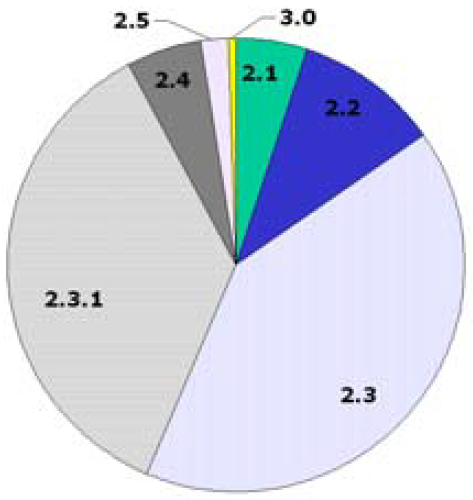
\includegraphics[width=0.35\textwidth]{HL7-versions-comparasion}
\caption[Approximate real-world usage of HL7 messaging standards]{Approximate real-world usage of HL7 messaging standards~\citep{Shaver2010}}
\label{fig:hl7-version-comparasion}
\end{figure}


\subsubsection{HL7 Messaging Standard Version 2} \label{sec:hl7-v2}

The HL7 v2 is a standard created several years ago. Nevertheless, it had evolving into some new versions. Currently, HL7 v2 is at version 2.7. However, as it was designed as backwards compatible, the version is not so relevant. In fact, what is often more important is how the system which is sending the message is populating the fields and segments the standard defines. 

The HL7 v2 stands as a simple protocol for exchanging clinical data and it stands as the most widely used healthcare information standard~\citep{Eichelberg2005}. Certainly, one reason for that is that the referred messages are plain text, with several fields split by the vertical slash character `|' as it is possible to observe in Figure~\ref{fig:hl7v2-msg}.

\addtocounter{footnote}{1}
\begin{figure}[t]
\centering
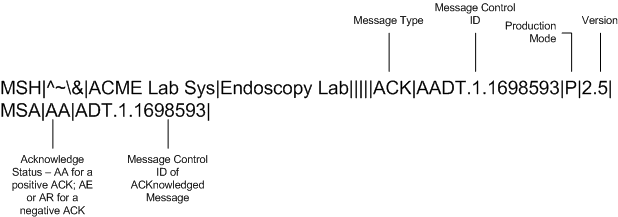
\includegraphics[width=0.9\textwidth]{HL7V2Message}
\caption[Example of an HL7 v2 acknowledgement message]{Example of an HL7 v2 acknowledgement message$^{\decimal{footnote}}$}
\label{fig:hl7v2-msg}
\end{figure}
\footnotetext[\value{footnote}]{Source: \url{http://www.interfaceware.com/images/ACKMessageAnatomy.png}}

However, some authors advocate that ``the messages lack a formal underlying reference model, and feature considerable optionality in addition to permitting user-defined elements''. In fact, that excessive flexibility obliges to establish a prior agreement structure and interpretation that might be called ``negotiated interoperability''~\citep{Atalag2010}. Obviously, this vagueness ``provides great flexibility but necessitates detailed bilateral agreements among the healthcare systems to achieve interoperability'' as state Eichelberg \textit{et al}~\citep{Eichelberg2005}.

In this context, it is important to clearly identify the main advantages of using HL7 v2, which we point out next~\citep{Atalag2010}:
\begin{itemize}
\item richly expressive data types;
\item support for arbitrary structured objects;
\item easy to adopt and use with low cost.
\end{itemize}

As expected, there are some arguments against also, which are:
\begin{itemize}
\item excessive flexibility and optionally in message interpretation implies a  ``negotiated interoperability'';
\item lack of privacy and consent guarantees;
\item growing tendency to abandon v2 in favour of v3. 
\end{itemize}

To conclude, despite of being an exceeded standard it is still very relevant, being used world wide. 

\subsubsection{HL7 Messaging Standard Version 3}

The HL7 v3 appeared as a natural evolution of HL7 v2, trying to solve some problems that the previous version had. Its first version was launched in 2005. Despite of being just a new release, this update means significant standard modifications as the main objective was to ``establish semantic interoperability in loosely coupled systems''~\citep{Atalag2010}. In this sense, at the core of this standard just appeared the Reference Information Model (RIM).

The RIM is an object model created as part of the Version 3 methodology, serving as a context provider to the multiple healthcare concepts. For instance, a WBC (white blood count) may refer to an order (intent) or a result (observation). In that case, the RIM structures ``implement the context by binding the coded vocabulary term from the ontology to a specific place in the model''~\citep{Shafarman2004}.

With HL7 v3, the messages are no longer plain text but XML files (as we can see in Figure~\ref{fig:hl7v3example}) which turns the message more human-readable but also more structured and rigid.

\begin{figure}[t]
\centering
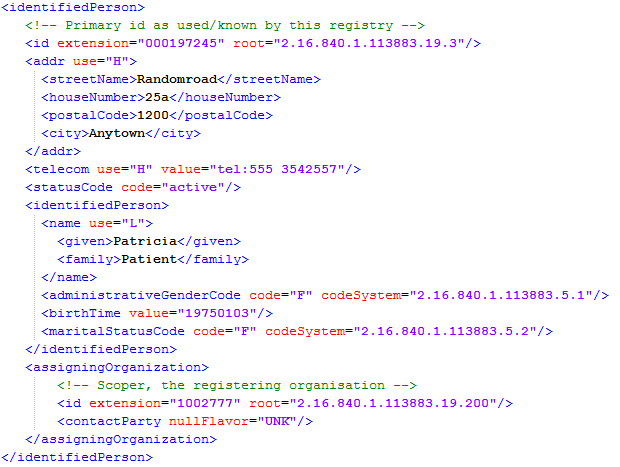
\includegraphics[width=0.86\textwidth]{hl7v3example}
\caption[Example of an HL7 v3 message]{Example of an HL7 v3 message~\citep{Spronk2007}}
\label{fig:hl7v3example}
\end{figure}

There are some advantages that should be credited to this Version 3, which are important to summarize~\citep{Atalag2010,Shaver2010}:
\begin{itemize}
\item rich in clinical semantics;
\item address many of the practical difficulties such as incomplete information, uncertainty, duplicate records and so forth;
\item dynamic model no more complex than v2;
\item ``less expensive to build and maintain mid-to-long term interfaces'';
\item ``more of a `true standard' and less `framework for negotiation''';
\item the long journey of maturing and reflecting about the standard.
\end{itemize}

Notwithstanding of the several advantages, there are some drawbacks that can be identified~\citep{Atalag2010,Shaver2010}:
\begin{itemize}
\item not clear where the return of investment is since it does not offers substantial advantages over v2 for some areas (simple alerting, drug interaction checking, recall systems, best practice guidelines, clinical pathways, and so forth);
\item message structures complex and difficult to understand;
\item ``inconsistencies between an Information Model (objects document things) interpretation and a Reference Ontology (objects are things) interpretation'';
\item not suitable as a model for storage EHR information and does not specify and EHR Architecture neither;
\item unclear how is it possible to query a v3 messages repository;
\item absence of compatibility with HL7 v2; 
\item expensive and slow adoption.
\end{itemize}

In an interesting research by Gartner in 2006, Rishel predicted that ``the HL7 V3 messages will fail to achieve critical mass, being replaced by ever-more-elaborate use of V2, a series of dialects of V3 chosen by individual countries and large enterprises, or the work of other standards organizations that may achieve less semantic interoperability while being easier to implement''~\citep{Rishel2006}.

To complete, the HL7 v3 seems the natural evolution for the applications using the previous versions. Although, that migration will take many years and it might not be so pacific as would be desirable.


\subsubsection{Clinical Document Architecture (CDA)} \label{sec:hl7-cda}
Clinical Document Architecture (CDA) is an ANSI-certified standard from HL7 organization. The first version (Release 1.0) was released in November, 2000 and the second (Release 2.0) was published with the HL7 2005 Normative Edition.~\citep{Seven} CDA defines the semantic and structure of clinical documents aiming to allow its exchanging. The CDA documents are actually XML documents. That concept is derived from the fact that these documents ``derive their meaning from the HL7 Reference Information Model (RIM) and use the HL7 Version 3 Data Types which are part of the HL7 RIM''~\citep{Atalag2010}.

The CDA document is constituted by two parts, an header and a body. The header is used to unambiguously state the semantics of each entry in the document. The body ``contains the clinical document content and can be either an unstructured text, or comprised of nested containers''~\citep{Eichelberg2005}.

It is important to distinguish the two versions of this standard, since there are many applications that still use the first version. The main characteristic of CDA standard is the documents classification into three different levels, although the interpretation of them is differentiated between the two versions.

The CDA Release One considers two levels~\citep{Seven,Eichelberg2005}:
\begin{itemize}
\item Level One --- basically it has a standardized header and additional information on the rest of the document;
\item Level Two --- allows to define and constraint both the structure and the content of the document, favouring the interoperability between systems since the receiver knows what to interpret;
\end{itemize}

The approximation of CDA Release Two is a little different. In fact, it provides an incremental approach, allowing and encouraging the documents to evolve and becoming more structured. One of the major additions is that the CDA body ``uses RIM structures and controlled vocabulary to permit a much higher level of semantic interoperability''~\citep{Seven}. Atalag \textit{et al} advocate that it is a ``stable and flexible standard for developing communications with coded information'' as well as ``provides a pathway from narrative free text documents through incrementally coded data to fully coded and semantically interoperable clinical data''~\citep{Atalag2010}.



\subsection{The openEHR} \label{sec:openehr}

The openEHR standard is a standard owned by the openEHR Foundation, created in 2002. The Foundation is a non-for-profit organization with the founding partners being University College London and Ocean Informatics, an Australian company. The main objective is to research and develop interoperable electronic health records related topics, aiming to improve the care quality to patients~\citep{Leslie2007}.

Unlike other standards, openEHR develops specifications for implementing full EHR systems, pronouncing more in persistence as opposed to messaging. openEHR states that, in order to achieve lifelong, patient centred, secure and shareable EHR, the way cannot be the aggregation of messages~\citep{Beale2002}.

In order to provide an high level of interoperability, openEHR suggests the engaging of standardized clinical content models (called Archetypes), a stable reference model and semantically rich terminologies~\citep{Atalag2010}. More in detail, Bale advocated a two-level methodology to model the EHR structure. In the first level, the existence of a generic reference model, specific to the healthcare domain but sufficiently general to be stable over the time (e.g. role, act, entity and so forth). In the second level, there were concepts mapped as archetypes, such as blood pressure, laboratory results and so on. The archetypes apply ``constraint rules  that specialize the generic data structures that can be implemented using the reference model''~\citep{Beale2002}.

Beyond the reference information model, the openEHR framework includes other resources that help the implementation following this standard, such as the ADL (Archetype Definition Language) language for expressing archetypes, an archetype library and a collection of open source implementations. As an example (Figure~\ref{fig:openehr-adl}), we can restrict a generic Observation class to, for example, a Blood Pressure archetype.

\begin{figure}[t]
\centering
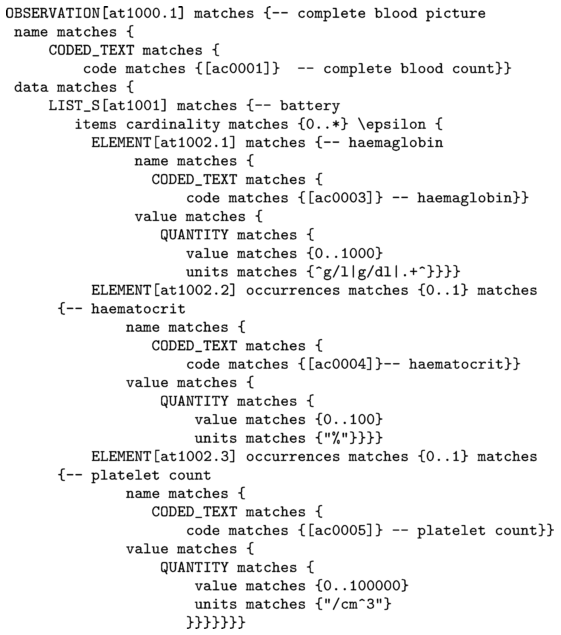
\includegraphics[width=0.7\textwidth]{openehr-adl}
\caption[The ADL definition of Complete Blood Count archetype]{The ADL definition of Complete Blood Count archetype ~\citep{Eichelberg2005}}
\label{fig:openehr-adl}
\end{figure}



\subsubsection{Advantages and Disadvantages}

There are some interesting characteristics about openEHR that might be useful to underline~\citep{Atalag2010}:
\begin{itemize}
\item intuitive and understandable model for clinicians;
\item approach based on recording and querying observations;
\item extracts can be sent with HL7 v2 (see~\ref{sec:hl7-v2});
\item likely stable reference model	over the time;
\item possibility to convert archetypes into CDA documents (see~\ref{sec:hl7-cda}).
\end{itemize}

On the other hand, Atalag \textit{et al} identified some arguments against either~\citep{Atalag2010}:
\begin{itemize}
\item ``lacks semantic rigour and does not contain a logically sound ontology'';
\item works well with simple scenarios, but does not easily handle complexity;
\item no experiences with medium to large-scale systems;
\item weak governance of the openEHR Foundation.
\end{itemize}

To conclude, the interest with this standard is spreading worldwide. There is an increasing number of full or partial implementations of the openEHR specifications in several countries, like United Kingdom, Sweden, Australia, Denmark, The Netherlands, Singapore, USA, Japan, Brazil, Scotland or Turkey. However, there is not a really large-scale systems in neither of these countries and the use of the standard consists of using some of its concepts~\citep{Atalag2010}. In another interesting article, Marta Silva and José Carvalho state that the ``openEHR standard has original and sound fundamental
concepts that definitely will influence future generations of health information systems'' as long as note that ``some openEHR core beliefs are highly debatable''. Also, they raise some questions about the applicability of semantic interoperability ``when the industry all over the world is struggling in exchanging basic unstructured demographic and clinical data through the complex network of health providers''.~\citep{SilvaMarta;Carvalho2011}




\subsection{Digital Imaging and Communications in Medicine} \label{sec:dicom}

DICOM (Digital Imaging and Communications in Medicine) is an worldwide used standard for medical image communication. The standard provides data structures and services allowing the exchange of medical images and related information. In the actual structure, the standard is available since 1993, despite the creation remounts to 1983.

Unlike most of other EHR standards, the DICOM uses a binary encoding. Pianykh has an interesting point of view, saying that ``contrary to popular belief, DICOM is not just an image or file format'' but ``an all-encompassing data transfer, storage, and display protocol built and designed to cover all functional aspects of digital medical imaging''~\citep{Pianykh2008}.

Other authors stated that ``it has become a leading standard used by all major vendors of diagnostic medical equipment'', predicting also that ``DICOM will soon be used in every medical branch that utilizes imaging, for example: cardiology, mammography, radiology, surgery, endoscopy, dentistry, pathology, etc''~\citep{Mustra2008}.


\subsection{Terminology and Ontology Standards}

The need of data sharing between different healthcare institutions leverage the creation of multiple standards, attempting to allow, not only the data sharing, but also the easy interpretation of the message's content. in fact, this kind of internationally endorsed classifications facilitate the storage, retrieval analysis and interpretation of data. In this sense, in the next subsections we will present some terminologies that were created with the aim of making the systems understand each other.

\subsubsection{Systematized Nomenclature of Medicine - Clinical Terms} \label{sec:snomed}

SNOMED CT (Systematized Nomenclature of Medicine - Clinical Terms) was created in 2006 by the International Health Terminology Standards Development Organisation (IHTSDO). This standard aims to provide a unique and embracing system with clinical terms. The objective is to have a repository, managed and updated centrally, available to all systems which adopted it and that can be used either to clinical purposes as to research projects.~\citep{ACSS/MS2009a}

Citing the official site, the SNOMED CT ``provides the core general terminology for the electronic health record (EHR) and contains more than 311,000 active concepts with unique meanings and formal logic-based definitions organized into hierarchies'' and ``can be used to represent clinically relevant information consistently, reliably and comprehensively as an integral part of producing electronic health records''~\citep{IHTSDO}.


\subsubsection{International Classification of Diseases} \label{sec:icd}

The International Classification of Diseases (ICD)~\citep{WHO} is ``the international standard diagnostic classification for all general epidemiological, many health management purposes and clinical use''. This standard is owned by the World Health Organization (WHO) and dates from 1850, being developed and reviewed every ten years. Although, every year new updated are release to the versions in use. The ICD provides an huge variety of codes to classify diseases, body signals, symptoms, abnormal aspects, complaints, social circumstances and external causes of injury or illness, beyond to having an additional classification used to classification of transplants and newborns and so forth. 

ICD is a classification, and a essential one, as it define the universe of entities to be studied, and highlight the relevant aspects of the information that has been collected. Also, it allows their comparison in several contexts: within and between populations over time and the compilation of internationally consistent data.

%TODO Logical Observations Identifiers Names and Codes (LOINC)

%\subsection{Overview}

%TODO meter tabela com comparação de standards como tem o lucas ribeiro






%%========================================
%% Internacional case studies
%%========================================

\section{International Case Studies}

Several Electronic Health Record projects were initiated in multiple countries. The study of same of those might be fundamental in order to understand what can we learn with them. By doing that, it will help us to extend our horizons, retain the bad experiences and better evaluate some options that we might have to take.

In the next subsections, we will provide an overview by two EHR initiatives: the Canada Health Infoway and the National Health Service (from England).

\subsection{Canada Health Infoway}

Canada Health Infoway is an non-for-profit organization founded by Canada's First Ministers in 2001. It was specifically created to accelerate the process of development of Electronic Heath Record systems, promoting the adoption of standards that guide to communication facilitation between different healthcare organizations. 

In order to guide the development of the systems in each different province, Infoway provided a national framework called EHR Blueprint. The EHR Blueprint is a set of principles, guides and components. It states ``a comprehensive description of the components necessary for the interoperable EHR and describes, in broad terms, how the components are envisioned to work together''~\citep{April2006}.

\subsubsection{Sharing EHR Information} \label{sec:share-ehri}
In the process of building an EHR, there are several methods to allow sharing EHR information along several services, consumers and providers. EHRS Blueprint advocates that the best method (at least for their reality) is the creation of a shared reference information source that is populated by several health-care organizations around Canada. This reference is populated with clinical relevant data and is maintained externally from ever health-care organization (or Points of Service, as designated in EHRS Blueprint). The Points of Service (PoS) are able to reference or pull data from the shared repository.

The `EHR Infostructure' is based on achieving full integration and interoperability between the EHR Solution and each PoS. In order to do so, EHRS Blueprint has a Health Information Access Layer that provides the interface which all the PoS communicate with. However, since EHRS Blueprint defines an unique interface for all PoS, most of these systems needed to adapt themselves to respect the standards and be able to stay connected to the system. 

This shared reference presupposes the existence of peers along each different Canada's jurisdiction. These peers represent several copies of the EHRi in terms of structure, but dealing only with the local PoS. As the infrastructure is the same, the process of retrieving information from other peers, when needed, is relatively simple.


\subsubsection{Architectural principles}

The EHRS Blueprint states~\citep{April2006} some architectural principles which guided the EHRs implementation. However, we will just point out the ones that might be more relevant and interesting at this point.

The fact of the EHR Infostructure information being stored as copy of the original one is a key characteristic, as it preserves independence between the EHRi and the PoS.

Another relevant principle is the controlled environment built around the system, defining one common interface and transforming EHRi into a black-box in which PoS can retrieve but also update clinical information for a specific patient.

The EHRS Blueprint was built following an Services Oriented Architecture, making the architecture more flexible and the components reusable. 

Another interesting fact is that there is no single `home' for the patient's electronic health record. Actually, each jurisdiction's EHRi holds and owns the data generated in health services from that jurisdiction.

\subsubsection{Key elements}

The EHR Blueprint has multiple components with certain characteristics. Although some of those had been already referred, it is useful to take a deeper look at them and point out some others also. Thus, the key elements are~\citep{April2006}:

\begin{figure}[t]
\centering
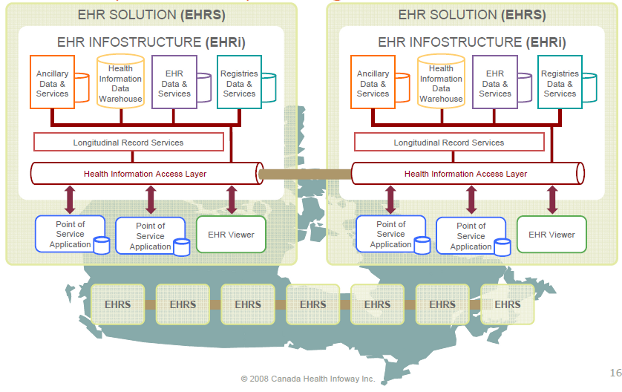
\includegraphics[width=1.0\textwidth]{blueprint-architecture}
\caption[EHRS Blueprint Architecture overview]%
			{EHRS Blueprint Architecture overview~\citep{Infoway}}
\end{figure}

\begin{itemize}
\item \textbf{Point of Service Applications (PoS)} --- these are software applications or information systems that provide clinical information to the EHR system, working as gateway for gathering critical patient data, absolutely fundamental to the system's purposes. It is important to notice that these systems are responsible for most collection of the patient's EHR data. Here, we refer to applications as an information system in hospital emergency department as well as an local pharmacy system and further so;

\item \textbf{EHR Data Repositories} --- sometimes, there is relevant clinical information that is no available in the PoS applications despite of being very relevant in a clinical decision making context. Instead, it is usually available through other systems. In this sense, the PoS applications are also responsible for pushing the data into these EHR Data Repositories -- that become responsible for storing it and keeping it available to the users that might need that. Four logical clinical domain repositories are identified by EHRS Blueprint: Shared Health Record, Drug Information, Diagnostic Imaging and Laboratory;

\item \textbf{Registry Services} --- there are the information linkers. There Registry Services provides the identification of patients, matching them with the required clinical data. In order to guarantee the match of required and retrieved information, these services offer: Client Registry, Provider Registry, Location Registry and Terminology Registry;

\item \textbf{Longitudinal Record Services (LRS)} --- as we saw in Subsection~\ref{sec:share-ehri}, the EHRS Blueprint is based on distributed data repositories. Thus, when it is needed to retrieve and show the information to the user (for instance, a physician), all the data must be gathered as if it was stored in the same place. These Longitudinal Record Services execute that task, bringing together data from different registries and sources, normalizing it for common understanding;

\item \textbf{Health Information Access Layer (HIAL)} --- it provides a single standardized way of sharing and retrieving data from EHRi. The fact of being unique and the single entry point obligates the PoS applications to adapt themselves to the interface but also to the information standards also. 
\end{itemize}


\subsection{England National Health Service}

The National Health Service (NHS) Connecting for Health is part of the UK Department of Health. This organization was created on 1 April 2005 as the replacement for an older one (NHS Information Authority). It has the responsibility of managing and implementing the NHS National Programme for IT (NPfIT). The NPfIT was an initiative to upgrade the NHS to a centrally-mandated electronic health record  for patients, connecting hundreds of hospitals and thousands of healthcare professionals and providing them relevant patient data by secure and certified means.


\subsubsection{Architecture overview}

The NPfIT has born as the world's largest civil information technology project, committing £12.4 billion over 10 years in order to improve the quality of healthcare in England. As expected, such a big project could not be just a single standalone implementation. In fact, the NPfIT is made of eight separated systems, which are~\citep{Brennan2005}: 
\begin{itemize}
\item \textbf{One National Application Service Provider (NASP)} --- designed to support the `National Data Spine', which was destined to keep the patients' electronic data;
\item \textbf{A New National Network (N3)} --- a network connecting all the hospitals, applications and other healthcare providers, characterized by the need of being a really broadband one. It would be an essential infrastructure supporting and linking all the other services providers;
\item \textbf{One Electronic Appointment Booking (eB)} --- a service (now called `Choose and Book') that would give the possibility of the patients to choose the place, date and time for their appointments in a hospital or clinic;
\item \textbf{Five Local Service Provider (LSP)} --- five physically distributed providers, hosting the NHS Care Records Service (NHS-CRS) at a local level, covering all England's territory.
\end{itemize}

\begin{figure}[t]
\centering
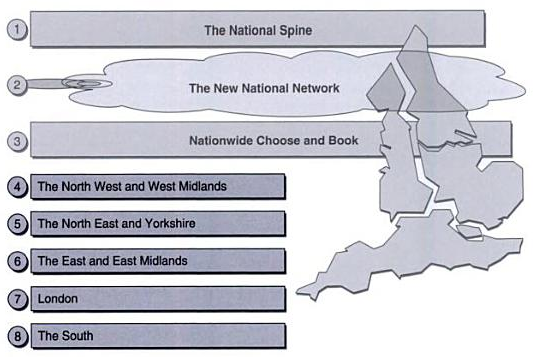
\includegraphics[width=0.7\textwidth]{npfit-architecture}
\caption[The England's National Programme for IT]{The England's National Programme for IT~\citep{Brennan2005}}
\label{fig:npfit-architecture}
\end{figure}

The Figure~\ref{fig:npfit-architecture} briefly describes the kind of interaction between the different components of the system. It is important to notice that, in order to implement the five local clusters, five providers were contracted and made responsible for delivering the local services. The idea was that, in one hand, the providers would be challenged to compete between each other, speeding up the process of implementation. On the other hand, the risk would be lower since there was different suppliers implementing similar systems in parallel. CSC Alliance, BT Health London, Accenture and The Fujitsu Alliance were the contracted LSP's for the main body of the programme.


\subsubsection{NHS Interoperability Toolkit (ITK)}
The NHS Interoperability Toolkit is a set of standards, frameworks and implementation guides to support and favour the interoperability between local systems and across them. The NHS ITK aims to support flexibility and local innovation and also removing barriers to entry. It also wants to be an enabler of evolution and reusing of solutions that already proved to be valuable, connecting all the peers by standardization in order to ensure that there are no silos being created.

One of the key concepts of ITK is the use of a maturity-based approach, allowing the organizations to evolve through small steps, particularly for CDA documents. The step-by-step maturity model allows the organization to incrementally progress from sharing binary data to sharing fully-coded CDA documents.

\begin{figure}[t]
\centering
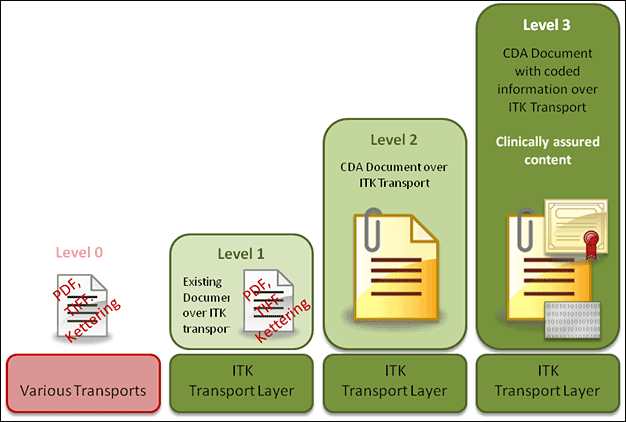
\includegraphics[width=0.8\textwidth]{itk-maturitymodel}
\caption[The NHS ITK Maturity Model]{The NHS ITK Maturity Model~\citep{Health2012}}
\label{fig:npfit-itk}
\end{figure}

As it is possible to observe in Figure~\ref{fig:npfit-itk}, there are four possible levels in the model. The lowest one -- Level 0 -- is applied to any organization, when even the sharing itself is made out of the ITK Transport Layer. When one organization becomes to use the ITK Transport Layer it reaches the Level 1. Then, the Level 3 is assigned when an organization is able to share CDA documents. Finally, when the data is passed through CDA documents one organization has reached the highest level -- Level 4. In Section~\ref{sec:hl7-cda} we explain the CDA standard more in detail.


\subsubsection{NHS Care Records}
The NHS Care Records is one of the NPfIT's components. This component is what we usually call an Electronic Health Record system, aiming to provide personal clinical information to the healthcare providers, increasing the quality and efficiency of the treatments.

The NHS Care Records considers two different types of records:
\begin{itemize}
\item \textbf{Summary Care Records} --- records held nationally. A Summary Care Record -- usually called Patient Summary -- stores essential information about a person, available in emergency situations, informing the health professionals about what medicines are one taking, the allergies that might suffer from or any known bad reactions to other medicines;
\item \textbf{Detailed Care Records} --- records held locally. The Detailed Care Record is a more comprehensive record which might store data from past exams and details, avoiding the necessity for repeating them, for example.
\end{itemize} 


\subsubsection{The fall and the failure}
The NPfIT started in October 2002 and since then it always been the target of some criticises. However, in April 2006, a set of 23 academics, wrote an open letter\footnote{Details: \url{http://editthis.info/nhs_it_info/The_Open_Letter_to_the_Health_Select_Committee}} raising several questions and concerns about the programme. A report by the King's Fund in 2007 also criticised the government's ``apparent reluctance to audit and evaluate the programme'', questioning their failure to develop a capable strategy~\citep{Wanless2007}.

The next years were very troubled as long as several reports raising doubts about the feasibility of the project were made public ~\citep{Powell2004,Coiera2007,Brennan2007,Clegg2007,Brennan2009}. One of those, by the Public Accounts Committee, stated in 2009 that the risks for the programme deployment were ``as serious as ever'', bringing up serious uncertainty about the capacity of the systems to meet expectations of clinical staff. \footnote{Details: \url{http://news.bbc.co.uk/2/hi/health/7850619.stm}} The over-and-over delays to deliver the fundamental services and the overrun of the programme's cost started to being unsupportable. In September 2011, the NPfIT has been dismantled following the conclusions of a new review by the Cabinet Office's Major Projects Authority (MPA)~\citep{OfHealth}.

 
\chapter{Architectural Proposal} \label{chap:arch-proposal}

\section*{}

This dissertation pretends to deliver an Architectural Proposal for the EHR. In that sense, this chapter is a briefly overview about how the work will be structured and the fundamental questions that must be answered in the end of this dissertation project.

\section{General architecture}

At this point, there are three essential questions that resume the work to be done:
\begin{itemize}
\item How to align the technology and business visions, allowing future evolution of the system?
\item Which data will be stored where?
\item Which standards will be used to format data and exchange information?
\end{itemize}

The problem of align the technology and business visions is one the greatest problems when talking about ultra-large scale software projects, as it was already referred in Section~\ref{sec:ea-frams}. The solution will probably come from the intersection of recommendations from the several Enterprise Architecture frameworks referred.

As the EHR is supposed to be a long-term project, the necessity for evolution will be a constant through the years. In that sense, it is critical that the architecture proposal allow and promote that evolution. Some approaches that might be helpful were described in Section~\ref{sec:arch-styles}.

The amount of information that is produced and stored, every day, by the healthcare organizations is enormous. This information can be classified by importance level what can give us an idea about which data is the most relevant and must be always available. Thus, the relevant information storing is a nuclear issue, as it can vary from a totally centrally-based approach to a complete distributed one.

To conclude, the way information is shared around the `players' includes the definition of: how to transmit the data, how to interpret the data and how to store the data. Basically, the problem starts with putting the systems to share information. Then, it is also required that the information transmitted can be understandable by the receiver. Finally, the way the information is stored, either centrally or in each institution is critical to facilitate all the integration.


\section{Work plan}

A work plan was created to guide the dissertation research work and is expressed in Figure~\ref{fig:workplan}.
The plan was divided in several tasks:
\begin{itemize}
\item International standards --- the first weeks will be necessary to study some of the standards internationally adopted, helping to understand better the EHR needs in terms of information standards;
\item Service-Oriented Architectures --- research about the implementation of this type of services in the health context and its applicability to the EHR;
\item Governance Model --- some time dedicated to study how it will be possible to manage all the system, maintaining the data integrity while allowing evolution;
\item Applications Architecture --- the requirements that allow new systems to be integrated and share information with the existing ones;
\item Architecture Proposal --- the proposal will be created over the time, along with the research;
\item Evaluate the Proposal --- evaluation with the study and application of some well-known methods;
\item Write and review thesis report --- finally, some time reserved to writing and reviewing the thesis document.
\end{itemize}

\mycustomfigure{workplan}{Dissertation work plan}{width=1.0\textwidth}
 
\chapter{Conclusions} \label{chap:concl}

%Deve ser apresentado um resumo do trabalho realizado e apreciada a
%satisfação dos objectivos do trabalho, uma lista de contribuições
%principais do trabalho e as direcções para trabalho futuro.
%
%A escrita deste capítulo deve ser orientada para a total compreeensãoo
%do trabalho, tendo em atenção que, depois de ler o Resumo e a
%Introdução, a maioria dos leitores passará à leitura deste capítulo de
%conclusões e recomendações para trabalho futuro.


The importance of an Electronic Health Record system and its benefits in the healthcare services equals the difficulty that they face to be implemented. In fact, this kind of platform take many years to be implemented, always resulting in high costs. In this context, it was important that this architecture proposal could reflect the existing case studies, in order to avoid approaches that could led to implementation failures. However, the challenges are not only the size of such project. Most of the times, EHR implementations have to deal with and manage multiple external factors, either political, economical or social. These factors tend to limit and condition the execution progress.


\section{General}

The health area has several actors, multiple institutions and not less business processes. In this scenario, it was fundamental that the research for designing the proposal was done close to the main stakeholders, essentially the healthcare organizations IT directors. On the other hand, the Portugal economic situation demands these projects to obtain short-term results. In this dissertation work, the main objective was not the short-term perspective but the long-term evolution and vision of the system. However, it was also important that the architecture proposal allows to obtain some quick results, without precluding the future development, not only because of the economic situation but also because that might be the right way to engage all the EHR stakeholders, from patients to healthcare organizations.

Throughout this dissertation study, an important knowledge of healthcare arena was gained. This knowledge is fundamental to be able to work in a complex context like this, where there are several stakeholders from completely different backgrounds, multiple institutions involved and many underlying interests. The research work was done on a weekly basis and in straight collaboration with the SPMS team. The existence of this cooperation allowed this work to be realistic. Moreover, it validates the dissertation work since that the people involved have many years of experience in the area and have a deep knowledge about the health information systems panorama and health organizations.

\section{Contributions}

The work done under this dissertation project comprehended several IT engineering areas. Indeed, the contribution was from the analyses of the business to understand the main requirements and problems, passing through the study of the information and application architecture, till the definition of a database model for the RCU2, with specific requisites to work over Oracle 7.3.1 databases.

Due to the research done, it was possible to state the possibility of making some little adjustments in order to facilitate and enhance future developments. In fact, there was always a concern about designing the architecture the right way but also to provide paths to quick-wins. In this sense, the authors believe that the main platform created to allow the data sharing (PDS) should focus on allow that. That is, the PDS should clearly stablish its limits and scope and then offer a set of services to provide the clinical data sharing following some principles of the Metropolis Model. This way, the user interfaces would be implemented by the consumers of the data, either hospitals or independent software companies, for instance. The point is that each consumer would integrate the data the way it wants. In addition, the availability of certified and secure open services would instigate the stakeholders to develop under those services, removing the need for government's investment and increasing the quality by competition.

Another conclusion is that there is an urgent need for normalisation. That is, the organizations must make an effort to normalise not only the codification standards but also the processes. However, the initiative and the example has to come from the higher instances under penalty of not being successful. On the other hand, in terms of standards, it is possible to say that the adoption of a standard to store and share clinical data will not solve all the problems but might be a pivotal step to solve several of them. Thereby, and following an evolutionary strategy, every interface or service thought to be available outside PDS, should be built with international standards, either for defining the services available (e.g. IHE profiles) as for encapsulate the data (e.g. HL7 CDA).

Regarding PDS internal organisation, it is recommended to use a SOA approach in order to improve flexibility and reuse of the multiple components and services. In this case, the immediate use of standards should be applied to the new services.

To conclude, the authors believe that the objectives were met and that the research constitutes an important document to alert the responsible entities to possible issues and new solutions.

\section{Future}

Despite of the effort that has already been spent and some positive results that have been achieved, there is still many changes to be done and many requirements to be met before Portugal can claim to have an EHR. Anyway, the path to reach it is too long and demands the existence of side projects that serve as guides and milestones of the global project.

The implementation and availability of the RCU2 should be the priority in the near future because it has potential to have an enormous positive impact. The authors believe that only the realization of this project is already a giant step to help the professionals increase of the healthcare services quality.

Apart from the conceptual and business challenges, the final purpose must guide all the future work: improving the patient healthcare services allowing the healthcare professionals to access relevant clinical information.
 

%%----------------------------------------
%% Final materials
%%----------------------------------------

\begin{singlespace}
  %% Bibliography
  %% Comment the next command if BibTeX file not used, 
  %% bibliography is in ``myrefs.bib''
  \PrintBib{webpages,myrefs}

  %% Index
  %% Uncomment next command if index is required,
  %% don't forget to run ``makeindex mieic'' command
  %\PrintIndex

  %% Comment next 2 commands if numbered appendixes not used
  \appendix
%  \chapter{RCU2 Database Model} \label{ap1:rcu2_db}

	
\end{singlespace}

\end{document}
